\section{Problem Statement}
%Nowadays, the energy crisis is a constant theme because of the inflated energy prices \cite{energy_crisis}. Furthermore, huge energy consumption is a burden to the environment, as not all means of energy production are non-polluting. According to "Our World in Data"\cite{owidenergy}, in 2019, 63,3\% of eletrical energy production comes from fossil fuels. It is known that, in cities, street lamps are continuously switched on at night, most of the time unnecessarily glowing with its full intensity in the absence of any activities in the street.  This leads to a great waste of energy, also contributing to the increase in light pollution. As claimed by National Geographic \cite{light_pollution}, 83\% of world population lives under light-polluted skies. This is a problem since it alters the biochemical rhythms that normally flow with natural light levels and also endangers ecosystems by harming animals whose life cycles depend on dark.
%
%With that in mind, the main objective of this project is the creation of a distributed system, composed by smart street lights capable of turning on only when they detect movement in the surroundings, at night time. 
Nowadays, the energy crisis is a constant theme because of the inflated energy prices \cite{energy_crisis}. Furthermore, huge energy consumption is a burden to the environment, as not all means of energy production are non-polluting. According to "Our World in Data"\cite{owidenergy}, in 2019, 63,3 \% of eletrical energy production comes from fossil fuels. It is known that, in cities, street lamps are continuously switched on at night, most of the time unnecessarily glowing with its full intensity, in the absence of any activities in the street, leading to a great waste of energy. Furthermore, it is in cities where the consequences of using cars are most noticeable. An example of this is the search for a parking space. According to the RAC Foundation [ref], in England, an average car is parked 95 \% of the time, which explains how hard it can get sometimes when trying to find a parking spot. This struggle leads to an increase in carbon dioxide production as well as fuel consumption.

With that in mind, the main objective of this project is the creation of a  distributed system, composed by smart street lights capable of turning on only when they detect movement in the surroundings, at night time, and also, capable of detecting available parking spaces in the street post vicinity.


\section{Problem Statement Analysis}
%In order to have a better and deeper understanding of the problem, it’s essential to identify the entities involved and their relationships. Using that analysis, a system diagram can be built, figure \ref{fig:Problem_statement_analysis}, relating the known entities and presenting some attributes.

%\begin{figure}[ht]
%	\centering
%	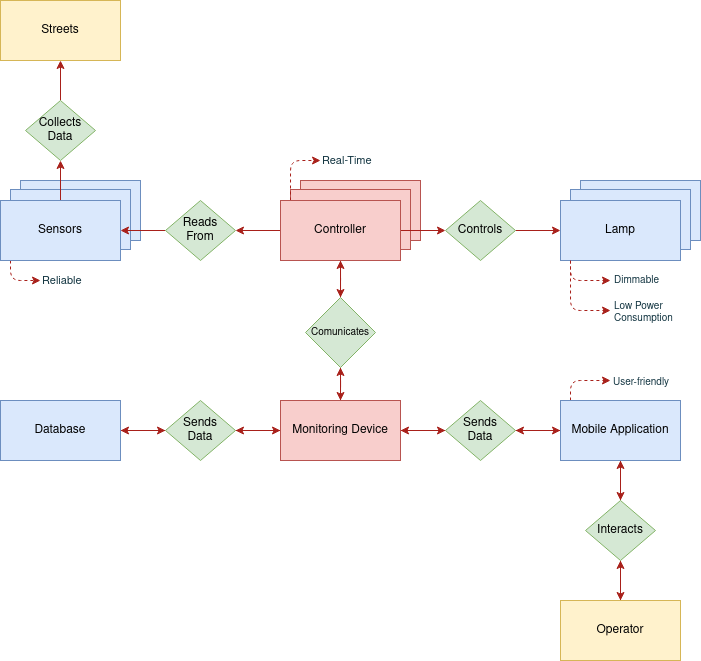
\includegraphics[width=1\textwidth]{Problem_statement_analysis}
%	\caption{Problem Statement Analysis Diagram.}
%	\label{fig:Problem_statement_analysis}
%\end{figure}

%The main purpose of this system is to control a street lamp, using Raspberry Pi 4B, turning the lamp on when movement in the surroundings is detected, only at night time. 
%
%Para a deteção do movimento, pode ser usada uma camera que, ao contrário de outros detetores de movimento, por exemplo os \ac{pir}, não é propensa a falsas deteções pois não são sensiveis a mudanças ambientais, como o fluxo de ar quente ou frio. Além disso, a camara permite a deteção de movimento nas redondezas de mais que um poste, diminuindo o número de sensores a utilizar. Por exemplo, se uma camera for capaz de detetar movimento nas redondezas de dois postes de luz, então seria necessário apenas uma camara, ao passo que, com sensores, seria necessária a sua colocação em todos os postes. Esta deteção deve ser realizada apenas de noite, sendo, para isso, necessário determinar as condiçoes de luminusidade do ambiente através de um sensor de luminusidade. De modo a facilitar a manutenção do poste, deve ser implementado um sistema que apura as condições de funcionamento da lâmpada. Quando este sistema verificar que a lâmpada não está em boas condiçoes de funcionamento, ou seja, que está partida ou fundida, esta informação deve ser transmitida à entidade responsável pela rede de postes de iluminação numa mensagem, enviada através de um modulo \ac{gsm}.
%
%The system consists of a monitoring device, which communicates with various controllers. Each controller manages a single light pole, ensuring that its lamp lights up whenever motion is detected, through its sensors. The monitoring device receives and sends data to a database, which contains information about all lamp posts, and communicates with a mobile application. A responsible person for the lamp posts network, the operator, uses the application to obtain knowledge about this network. In addition, the monitoring device can also request each controller to turn on their lamp, regardless of whether or not there is movement in the vicinity of this pole.
%
%Each street lamp post must communicate wirelessly with the neighbor lamp posts, allowing to dynamically turn on the lights of the following poles. Also, each smart street light must evaluate if its lamp is in good conditions and, when not verified, report to the responsible authority.
%
The main purpose of this system is to control a street lamppost, using Raspberry Pi 4B. When there is no activity in the area, the lamppost is at a pre-defined minimum light level, as when a car or pedestrian is noticed in the area, the light must automatically activate. Therefore, each street lamp post must communicate wirelessly with the neighbor lamp posts, allowing to dynamically turn on the lights of the following poles. To detect movement in the vicinity of the pole, a motion detector must be used, which must only work at night. To ensure this, a luminosity sensor can be used, determining the ambient light conditions. In order to facilitate the maintenance of the pole, a system that determines the operating conditions of the lamp must be implemented. When this system verifies that the lamp is not in good working conditions, that is, that it is broken or burnt, this information must be transmitted to the entity responsible for the network of lampposts through a mobile app. This should also be used by the person in charge, to manage all information on the pole network, such as the location of each pole, O QUE MAIS???. In order to allow the detection of parking spots, this system should only be used in an area where there are parking spaces nearby. For this, the lamppost must have a camera, turned on all day, and, after Raspberry processes the acquired information, it must be made available on a website, so that a user can know where parking spaces are available.